\documentclass[10pt,pdftex]{report}
\usepackage[T1]{fontenc}
\usepackage[utf8]{inputenc}
\usepackage[magyar]{babel}
\usepackage{graphicx}
\usepackage{amsmath}
\usepackage{amssymb}
\usepackage{multirow}
\usepackage{booktabs}
\usepackage{indentfirst}
\usepackage[a4paper]{geometry}
\usepackage{url}
\usepackage{titling}
\usepackage{float}
\usepackage{xcolor}
    \definecolor{titlebg}{RGB}{128,128,128}

\usepackage{lmodern}
\usepackage{etoolbox}
\patchcmd{\thebibliography}{\chapter*}{\section*}{}{}

\renewcommand{\thesection}{\arabic{section}}


\title{Ingamozgás mérése}

%% EZ ALÁBBI KÉT MEZŐT ÉRTELEMSZERŰEN KI KELL TÖLTENI
\author{Bíró Gergő Tamás}
\date{2025. március 18.}


%% FEJLÉC LEÍRÓ, NEM KELL MÓDOSÍTANI
\renewcommand*{\maketitle}{\noindent\colorbox{titlebg}{%
\parbox{\dimexpr\linewidth-2\fboxsep}{\color{white}%
\parbox{\linewidth}{\fontsize{18}{24}\selectfont\sffamily\bfseries\thetitle}%
}}\vskip 1em%
\begin{tabular}{l}%
Mérést végezte: \theauthor \\%
Mérés dátuma: \thedate\\
Jegyzőkönyv végleges változata: \today %
\end{tabular}%
}
%%%%%%%%%%%%%%%%%%%%%

\begin{document}
\maketitle

%% ÉRDEMI MUNKA HELYE
\section*{A mérés célja}
A mérés során a mikrokontroller által a szöghöz rendelt szám és a szög közötti kapcsolatot akarjuk meghatározni, majd a súrlódásos inga mozgását vizsgáljuk, ezután a 
lengés periódusidejének a kezdeti amplitúdófüggését határozzuk meg, majd végül az amplitúdó változásának a mértékét vizsgáljuk meg a kezdeti amplitúdó függvényében.
\section*{A mérési feladatok dokumentációja, az adatok kiértékelése és az eredmények értelmezése}
\subsection*{A mérés során használt eszközök}
\begin{itemize}
    \item{Keretben felfüggesztett inga.}
    \item{Rézpálca az inga egy pozícióban való kitámasztásához.}
    \item{Potencióméter.}
    \item{Gyorsulásmérő szenzor.}
    \item{MIkrokontroller, amely a potencióméter és a gyorsulásmérő adatait, valamint az időt rögzíti.}
\end{itemize}
\subsection*{A mérés leírása}
Először a potencióméter adatait akarjuk az inga kitérési szögével összekalibrálni, amelyhez először az inga nyugalmi állapotában nagyjából 10 másodpercig rögzítjük a gyorsulásmérő 
által mért adatokat, amelyből kiszámoljuk a nyugalmi gyorsulás egységvektorát. Ezután az ingát kitérítjük, és a sárgaréz pálca segítségével kitámasztjuk az akutális pozícióban. 
Miután az inga már nem rezeg szintén nagyjából tíz másodpercig mérjük a gyorsulási adatokat, amelyekből kiszámítjuk a gyorsulásának egységvektorát, és annnak szórását, ezt 
6-8 különböző kitérés mellet megtesszük. Ezután a kapott adatokból kiszámítjuk az egyes pozíciókhoz tartozó szöget, és egyenest illesztünk a szögekre a potencióméter által 
mért adatokból kapott szám föggvényében. Ezután már az inga lengését fogjuk vizsgálni, úgy hogy több különböző kitérés mellett elindítjuk az ingát, és a lengése során rögzítjük 
a potencióméter adataiból származó számot, amelyből a szöget kiszámítva a szögre a megfelelő alakú függvényt illesztünk. Ezek után az előzőleg kapott adatok alapján a periódusidő 
kezdeti amplitúdótól való függését akarjuk függvény illesztésével meghatározni, és végül az amplitúdó csillapításának a mértéke és a kezdeti amplitúdó közötti összefüggést vizsgáljuk meg.
\subsection*{A mérés kiértékelése}
\subsubsection*{Kitérés szögének kalibrálása}
A gyorsulás egységvektorának nyugalmi állapotban való meghatározásához a gyorsulási adatokat megközelítőleg 10.5$s$-ig mértük, a vektor egyes komponenseit az adott komponensre mért 
adatok átlagából, azok hibáját pedig az értékek szórásából határozzuk meg, majd ezeket a kapott gyorsulásvektor hosszával leosztjuk a nyugalmi gyorsulás egységvektora, és a hibájának 
a meghatározásához. A mérésből az egységvektorra a következő adódott:
\[
\mathbf{e_0}=
\begin{pmatrix}
    -0.051 \\
    0.0082 \\
    0.9987 
\end{pmatrix} \pm \begin{pmatrix}
    9.2\cdot 10^{-6} \\
    9.1\cdot 10^{-6} \\
    2.2\cdot 10^{-5}
\end{pmatrix}\frac{m}{s^2}
\]
Ezután ugyanezzel a módszerrel határozzuk meg a kitérítések során kapott egységvektorokat is, a feltűntetett $\mu_x$ mennyiség a potencióméterből kapott adatokból származó szám átlaga, $\sigma_x$ annak a hibája. A kapott értékek a következők:
\begin{table}[H]
    \centering
    \begin{tabular}{|r|r|r|r|}
        \hline
        $\mu_x$ & $\sigma_x$ & $\mathbf{e_{\Theta}}(\frac{m}{s^2})$ & $\Delta\mathbf{e_{\Theta}}(\frac{m}{s^2})$ \\
        \hline
        558.1 & 1.031 & $\begin{pmatrix} 0.104 \\ 0.280 \\ 0.954\end{pmatrix}$ & $\begin{pmatrix} 0.0032 \\ 0.0032 \\ 0.0045\end{pmatrix}$ \\
        \hline
        589.1 & 1.013 & $\begin{pmatrix} 0.154 \\ 0.371 \\ 0.916\end{pmatrix}$ & $\begin{pmatrix} 0.0038 \\ 0.0048 \\ 0.0045\end{pmatrix}$ \\
        \hline
        639.9 & 1.072 & $\begin{pmatrix} 0.233 \\ 0.513 \\ 0.826\end{pmatrix}$ & $\begin{pmatrix} 0.0039 \\ 0.0051 \\ 0.0047\end{pmatrix}$ \\
        \hline
        658.0 & 1.089 & $\begin{pmatrix} 0.260 \\ 0.558 \\ 0.788\end{pmatrix}$ & $\begin{pmatrix} 0.0031 \\ 0.0032 \\ 0.0046\end{pmatrix}$ \\
        \hline
        678.2 & 1.042 & $\begin{pmatrix} 0.287 \\ 0.607 \\ 0.741\end{pmatrix}$ & $\begin{pmatrix} 0.0035 \\ 0.0041 \\ 0.0047\end{pmatrix}$ \\
        \hline
        686.4 & 1.056 & $\begin{pmatrix} 0.304 \\ 0.634 \\ 0.712\end{pmatrix}$ & $\begin{pmatrix} 0.0035 \\ 0.0044 \\ 0.0047\end{pmatrix}$ \\
        \hline
        700.1 & 1.064 & $\begin{pmatrix} 0.319 \\ 0.662 \\ 0.678\end{pmatrix}$ & $\begin{pmatrix} 0.0032 \\ 0.0033 \\ 0.0047\end{pmatrix}$ \\
        \hline
        749.2 & 0.976 & $\begin{pmatrix} 0.380 \\ 0.767 \\ 0.516\end{pmatrix}$ & $\begin{pmatrix} 0.0032 \\ 0.0032 \\ 0.0047\end{pmatrix}$ \\
        \hline
        773.9 & 1.121 & $\begin{pmatrix} 0.404 \\ 0.808 \\ 0.430\end{pmatrix}$ & $\begin{pmatrix} 0.0032 \\ 0.0032 \\ 0.0046\end{pmatrix}$ \\
        \hline
        798.4 & 0.920 & $\begin{pmatrix} 0.427 \\ 0.846 \\ 0.318\end{pmatrix}$ & $\begin{pmatrix} 0.0030 \\ 0.0031 \\ 0.0047\end{pmatrix}$ \\
        \hline
    \end{tabular}
    \caption{Gyorulás egységvektora, x átlaga különböző méréseknél.}
\end{table}
A fentiekben az inga csak egy irányba lett kitérítve, az arra való kitérítés szöge legyen mostantól pozitív az ellenkező irányé pedig negatív. Ebben az esetben a kitérési szög 
kiszinuszát megkaphatjuk a két egységvektor skalárszorzataként, tehát a szöget a következő módon számolhatjuk ki:
\begin{equation*}
    \Theta = \arccos\left(\mathbf{e_0}\cdot\mathbf{e_{\Theta}}\right)
\end{equation*}
$\Theta$ hibáját pedig a következő képlet adja meg:
\begin{equation*}
    \centering
    \Delta\Theta = \frac{1}{\sqrt{1 - \left(\mathbf{e_0}\cdot\mathbf{e_{\Theta}}\right)^2}}\left(\left(\frac{\Delta\mathbf{e_{\Theta1}}}{\mathbf{e_{\Theta1}}}+\frac{\mathbf{\Delta e_{01}}}{\mathbf{e_{01}}}\right)\mathbf{e_{\Theta1}}\mathbf{e_{01}}
    +\left(\frac{\Delta\mathbf{e_{\Theta2}}}{\mathbf{e_{\Theta2}}}+\frac{\mathbf{\Delta e_{02}}}{\mathbf{e_{02}}}\right)\mathbf{e_{\Theta2}}\mathbf{e_{02}}+\left(\frac{\Delta\mathbf{e_{\Theta3}}}{\mathbf{e_{\Theta3}}}+\frac{\mathbf{\Delta e_{03}}}{\mathbf{e_{03}}}\right)\mathbf{e_{\Theta3}}\mathbf{e_{03}}\right)
\end{equation*}
Ezeket a képleteket alkalmazva a szög és annak hibája radiánban kifejezve a mért x értékek átlaga mellett a következők:
\begin{table}[H]
    \centering
    \begin{tabular}{|r|r|r|r|}
        \hline
        $\mu_x$ & $\sigma_x$ & $\Theta$ & $\Delta\Theta$ \\
        \hline
        558.1 & 1.031 & 0.3175 & 0.0140 \\
        \hline
        589.1 & 1.013 & 0.4288 & 0.0105 \\
        \hline
        639.9 & 1.072 & 0.6144 & 0.0079 \\
        \hline
        658.0 & 1.089 & 0.6785 & 0.0072 \\
        \hline
        678.2 & 1.042 & 0.7518 & 0.0066 \\
        \hline
        686.4 & 1.056 & 0.7949 & 0.0063 \\
        \hline
        700.1 & 1.064 & 0.8419 & 0.0061 \\
        \hline
        749.2 & 0.976 & 1.0441 & 0.0052 \\
        \hline
        773.9 & 1.121 & 1.1425 & 0.0049 \\
        \hline
        798.4 & 0.920 & 1.2628 & 0.0048 \\
        \hline
    \end{tabular}
    \caption{A szögek mérete radiánban a mért x értékek átlaga mellett.}
\end{table}
A fenti táblázatban látható adatokra lineáris összefüggést feltétellezve a következő függvényt illesztjük:
\begin{equation*}
    \Theta=ax+b
\end{equation*}
Ahol $\Theta$ a kitérés szöge radiánban, x a potencióméter adataiból kapott szám, $a$ és $b$ pedig az egyenes konstans paraméterei. Az illesztést a paraméterek hibáit 
figyelembe véve elvégezve a paraméterekre a következő adódik:
\begin{table}[H]
    \centering
    \begin{tabular}{|r|r|r|}
        \hline
        Paraméter neve & paraméter értéke & paraméter hibája \\
        \hline
        a & 0.00401 & $6.43\cdot 10^{-5}$ \\
        \hline
        b & -1.957 & $4.64\cdot 10^{-2}$ \\
        \hline
    \end{tabular}
    \caption{Az illesztés során kapott paraméterek, és hibájuk.}
\end{table}
A szögeket ábrázolva x függvényében a következő ábrát kapjuk:
\begin{figure}[H]
    \centering
    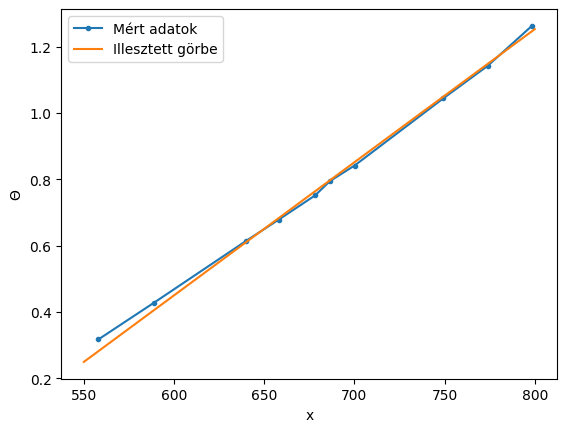
\includegraphics{./Kalibralas.png}
    \caption{$\Theta$ és $x$ kalibrációja}
\end{figure}
\subsubsection*{Normál lengés vizsgálata}
Az inga lengését különböző kezdeti kitérések mellett vizsgáljuk, az egyes mérések nagyjából 0.5-1 percig tartottak, azonban a kapott adatsorokból ki lettek vágva megközelítőleg 
3 periódus hosszú szakaszok azért, hogy megfelelő pontossággal lehessen az adatokra függvényt illeszteni, az egyes mérések során kapottadatokra. A vágás után megmaradt adatokra a 
következő függvényt illesztjük:
\begin{equation*}
    \Theta\left(t\right)=\Theta_0+\Theta_{max}\mathrm{e}^{-t/\tau}\sin\left(2\pi\frac{t}{T}+\Phi\right)
\end{equation*}
Ahol $\Theta\left(t\right)$ a kitérés szöge az időben radiánban kifejezve, $\Theta_0$ a rendszer nyugalmi állapotában mért kitérés, $\Theta_{max}$ a kezdeti maximális kitérés szöge, 
$t$ az idő, $\tau$ az az időtartam, amely alatt a kitérés az $\mathrm{e}$-ed részére csökken, $T$ a lengés periódusideje, $\Phi$ pedig a kezdeti fázisa. Az egyes lengésekhez az adott 
időpillanathoz a kitérés szögét a fentiekben látott $\Theta(x)$ összefüggés alapján számoljuk ki a rögzített $x$ adatokból. Az illesztést elvégezzük a vágodtt adatsorokon, amennyiben 
$\Theta_{max}$-ra negatív számot kapnánk, abban az esteben $\pi$ fáziseltolássla pozitívvá tennénk az amplitúdót, az így kapott paraméterek a következők:
\begin{table}[H]
    \centering
    \begin{tabular}{|r|r|r|r|r|r|}
        \hline
        Mérés száma & $\Theta_0$ & $\Theta_{max}$ & $\tau(s)$ & $T(s)$ & $\Phi$ \\
        \hline
        1. & -0.041 & 1.223 & 102.65 & 1.943 & 1.28 \\
        \hline
        2. & -0.043 & 1.089 & 104.78 & 1.905 & 1.31 \\
        \hline
        3. & -0.056 & 0.478 & 73.92 & 1.797 & 0.92 \\
        \hline
        4. & -0.062 & 0.275 & 52.61 & 1.780 & 2.32 \\
        \hline
        5. & -0.062 & 0.206 & 28.99 & 1.775 & 1.21 \\
        \hline
        6. & -0.049 & 0.813 & 94.82 & 1.844 & 1.61 \\
        \hline
        7. & -0.050 & 0.810 & 92.04 & 1.843 & 0.97 \\
        \hline
        8. & -0.052 & 0.684 & 85.35 & 1.822 & 1.41 \\
        \hline
        9. & -0.041 & 1.343 & 107.35 & 1.984 & 1.36 \\
        \hline
        10. & -0.045 & 0.972 & 107.72 & 1.877 & 1.29 \\
        \hline
        11. & -0.062 & 0.194 & 29.40 & 1.775 & 1.40 \\
        \hline
    \end{tabular}
    \caption{A lengésekre illesztett függvény paraméterei.}
\end{table}
A fenti paraméterek hibájára pedig a következők adódtak:
\begin{table}[H]
    \centering
    \begin{tabular}{|r|r|r|r|r|r|}
        \hline 
        Mérés száma & $\Delta\Theta_0$ & $\Delta\Theta_{max}$ & $\Delta\tau(s)$ & $\Delta T(s)$ & $\Delta\Phi$ \\
        \hline 
        1. & 0.00059 & 0.0016 & 3.96 & 0.00026 & 0.0015 \\
        \hline 
        2. & 0.00045 & 0.0012 & 3.64 & 0.00022 & 0.0012 \\
        \hline 
        3. & 0.00019 & 0.0005 & 1.84 & 0.00020 & 0.0013 \\
        \hline 
        4. & 0.00020 & 0.0006 & 1.94 & 0.00035 & 0.0020 \\
        \hline 
        5. & 0.00020 & 0.0005 & 0.71 & 0.00049 & 0.0030 \\
        \hline 
        6. & 0.00029 & 0.0008 & 2.71 & 0.00018 & 0.0010 \\
        \hline 
        7. & 0.00028 & 0.0007 & 2.37 & 0.00017 & 0.0010 \\
        \hline 
        8. & 0.00027 & 0.0007 & 2.45 & 0.00020 & 0.0012 \\
        \hline 
        9. & 0.00073 & 0.0020 & 4.84 & 0.00030 & 0.0016 \\
        \hline 
        10. & 0.00040 & 0.0011 & 3.88 & 0.00021 & 0.0012 \\
        \hline 
        11. & 0.00020 & 0.0001 & 0.82 & 0.00054 & 0.0032 \\
        \hline
    \end{tabular}
    \caption{A lengésekre illesztett függvény paramétereinek hibája.}
\end{table}
Az alábbiakban ábrázolva lesznek a mért adatok, és a hozzájuk tartozó illesztett függvények néhány mérés esetében.
\begin{figure}[H]
    \centering
    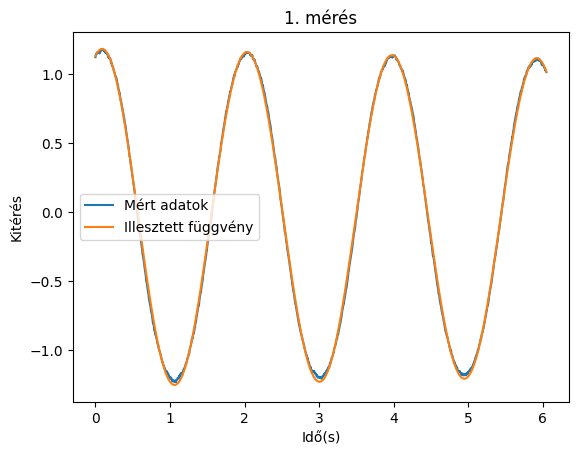
\includegraphics[scale=0.5]{./Lenges_1.png}
\end{figure}
\begin{figure}[H]
    \centering
    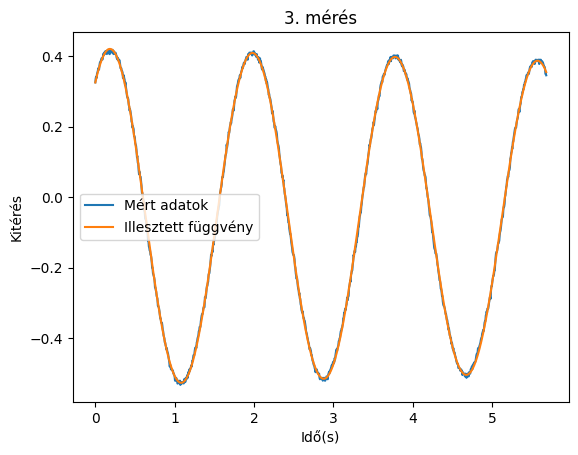
\includegraphics[scale=0.5]{./Lenges_2.png}
\end{figure}
\begin{figure}[H]
    \centering
    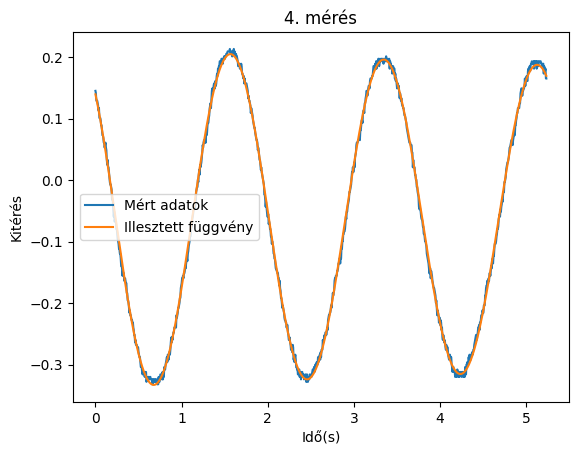
\includegraphics[scale=0.5]{./Lenges_3.png}
\end{figure}
\begin{figure}[H]
    \centering
    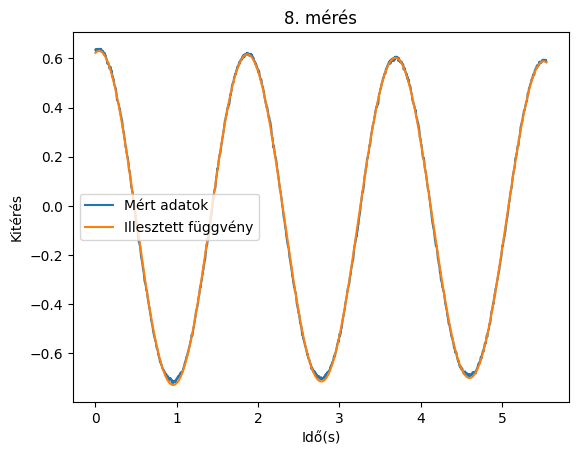
\includegraphics[scale=0.5]{./Lenges_4.png}
\end{figure}
\begin{figure}[H]
    \centering
    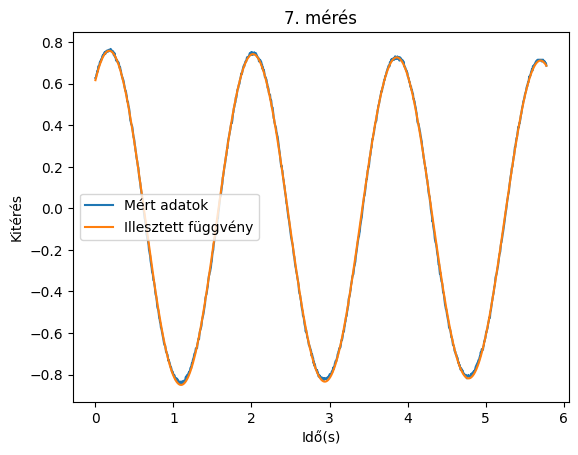
\includegraphics[scale=0.5]{./Lenges_5.png}
\end{figure}
\begin{figure}[H]
    \centering
    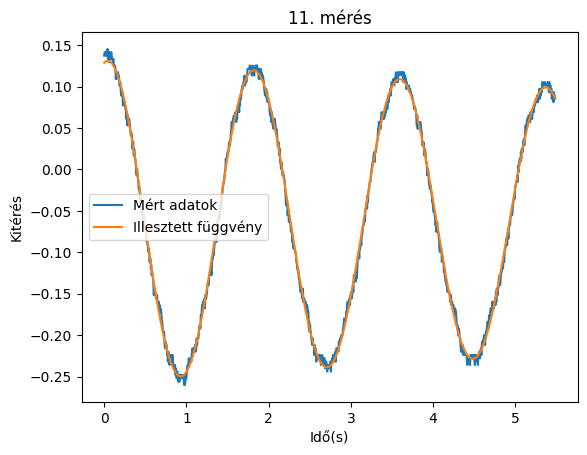
\includegraphics[scale=0.5]{./Lenges_6.png}
\end{figure}
\subsubsection*{A lengési idő amplitúdófüggésének vizsgálata}
Az alábbiakban az az előző feladatrészben kapott adatok alapján akarjuk igazonli a következő összefüggést:
\begin{equation*}
    T=T_0\left(1+\frac{\Theta^2_{max}}{16}+\mathcal{O}\left(4\right)\right)
\end{equation*}
Ahol $T$ a periódusidő, $T_0$ a "0 kitéréshez" tarrozó periódusidő, $\Theta_{max}$ a kezdeti amplitúdó, $\mathcal{O}(4)$ pedig a negyed és magasabb rendű tagok, amelyeket lehanyagolunk.
Ezt olyan módon akarjuk megtenni, hogy a következő föggvényt akarjuk illeszteni az adatainkra:
\begin{equation*}
    T=T_0\left(1+\frac{\Theta^2_{max}}{c}\right) 
\end{equation*}
Ahhol $a$ egy konstans osztó. Az illesztésből kapott függvényt majd az eredeti modellel akarjuk összehasonlítani. Az illesztés során $T$-t és $\Theta_{max}$-ot a lengés 
vizsgálata során kapott illesztési paraméterekből vesszük, az illesztés során  mind a két paraméter hibáját figyelembe vettük, az igy kapott értékek és hibájuk a paraméterekre:
\begin{table}[H]
    \centering
    \begin{tabular}{|r|r|r|}
        \hline
        Paraméter neve & paraméter értéke & paraméter hibája \\
        \hline
        c & 15.44 & $0.033$ \\
        \hline
        $T_0$ & 1.769$s$ & $1.6\cdot 10^{-4}s$ \\
        \hline
    \end{tabular}
    \caption{Az illesztés során kapott paraméterek, és hibájuk.}
\end{table}
Az alábbiakben látható az illesztett modell, az elméleti modell, és az eredeti adatpontok egymás mellett:
\begin{figure}[H]
    \centering
    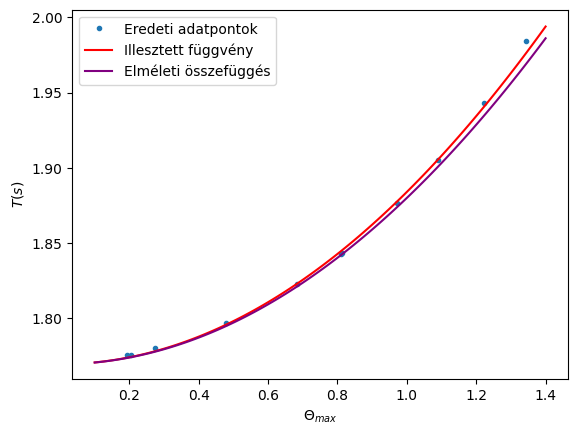
\includegraphics{./Periodusido.png}
    \caption{Az illesztett, és az elméleti modell a periódusidő amplitúdófüggésére.}
\end{figure}
Ahogy látható az illesztett, és az elméleti modell jó közelítéssel megegyeznek, azonbabn az illesztett függvény nagy amplitúdók esetén már láthatóan pontosabban illeszkedik a pontokra.
\subsubsection*{$\tau$ és $\Theta$ kapcsolata}
$\tau$-t ábrázolva $\Theta_{max}$ függvényében látható, hogy a köztük lévő összefüggés nem lineáris:
\begin{figure}[H]
    \centering
    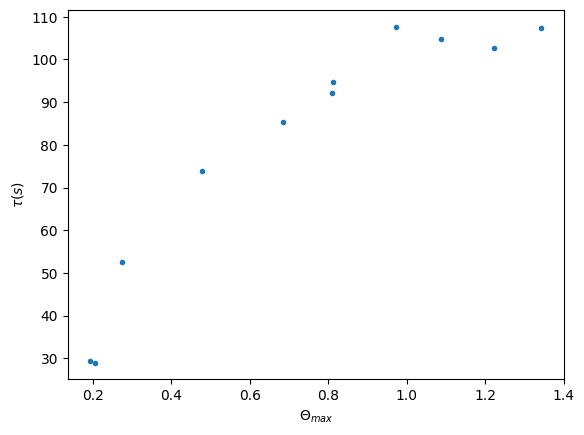
\includegraphics{./Tau.png}
    \caption{$\tau$ függése a $\Theta_{max}$-tól.}
\end{figure}
Azonban megfigyelhető, hogy $\tau$ $\Theta_{max}$ növekedésével szintén nő, ám ez a növekedés lelassul nagy amplitúdók esetén. Ez feltehetőleg azért történik, mert 
az amplitúdó növelésével a rendszer kezdteti energiája növekedni fog, méghozzá $E_{max}~1-\cos\left(\Theta_{max}\right)$ arányossággal, a csillapító erő, mivel súrlódási erő jó 
közelítéssel tekinthető konstansnak, azonban ennek az egy periódus alatt végzett munkája már függ $\Theta_{max}$-tól: $W~\Theta_{max}$, így valószínüleg $\tau$ növekedési mértékének a
lelassulása azzal magyarázható, hogy a kezdeti energia növekedése kisebb mértékű, mint az ingát fékező erő teljesítménye.
\section*{Összegzés}
A mérés során siekresen kalibráltuk a mikrokontrollel által adott $\Theta$-t a kitérés szögét a mikrokontrollel által rögzített x szábhoz, amelyet egy potencióméter feszültségéből generált. 
Ezután az inga lengését több kölönböző kezdeti amplitúdó mellett vizsgáltuk, amelyek néhány periódusára függvény illesztésével meghatároztuk a mozgás paramétereti, majd ezeket a 
paramétereket vizsgálva jó közelítéssel igazoltuk a periódusidő kezdeti amplitúdótól való függésére kapott összefüggést, valamint megvizsgáltuk az amplitúdó csökkenésének mértéke, 
a kezdeti amplitúdótól való függését.
%% IRODALOMJEGYZÉK
%\begin{thebibliography}{9}

%\bibitem{lamport94}
%  Leslie Lamport,
%  \textit{\LaTeX: a document preparation system},
%  Addison Wesley, Massachusetts,
%  2nd edition,
%  1994.
%  \url{https://bla.com}

%\end{thebibliography}

\end{document}
